% #######################################
% ########### FILL THESE IN #############
% #######################################
\def\mytitle{Coursework Report}
\def\mykeywords{Napier, SET09117, Algorithms, Data Structure, Steven, Gibson, 40270320, Steven Gibson, report}
\def\myauthor{Steven Gibson}
\def\contact{40270320@live.napier.ac.uk}
\def\mymodule{Module Title (SET09117)}
% #######################################
% #### YOU DON'T NEED TO TOUCH BELOW ####
% #######################################
\documentclass[10pt, a4paper]{article}
\usepackage[a4paper,outer=1.5cm,inner=1.5cm,top=1.75cm,bottom=1.5cm]{geometry}
\twocolumn
\usepackage{graphicx}
\graphicspath{{./images/}}
%colour our links, remove weird boxes
\usepackage[colorlinks,linkcolor={black},citecolor={blue!80!black},urlcolor={blue!80!black}]{hyperref}
%Stop indentation on new paragraphs
\usepackage[parfill]{parskip}
%% Arial-like font
\IfFileExists{uarial.sty}
{
    \usepackage[english]{babel}
    \usepackage[T1]{fontenc}
    \usepackage{uarial}
    \renewcommand{\familydefault}{\sfdefault}
}{
    \GenericError{}{Couldn't find Arial font}{ you may need to install 'nonfree' fonts on your system}{}
    \usepackage{lmodern}
    \renewcommand*\familydefault{\sfdefault}
}
%Napier logo top right
\usepackage{watermark}
%Lorem Ipusm dolor please don't leave any in you final report ;)
\usepackage{lipsum}
\usepackage{xcolor}
\usepackage{listings}
%give us the Capital H that we all know and love
\usepackage{float}
%tone down the line spacing after section titles
\usepackage{titlesec}
%Cool maths printing
\usepackage{amsmath}
%PseudoCode
\usepackage{algorithm2e}

\titlespacing{\subsection}{0pt}{\parskip}{-3pt}
\titlespacing{\subsubsection}{0pt}{\parskip}{-\parskip}
\titlespacing{\paragraph}{0pt}{\parskip}{\parskip}
\newcommand{\figuremacro}[5]{
    \begin{figure}[#1]
        \centering
        \includegraphics[width=#5\columnwidth]{#2}
        \caption[#3]{\textbf{#3}#4}
        \label{fig:#2}
    \end{figure}
}

\lstset{
	escapeinside={/*@}{@*/}, language=C++,
	basicstyle=\fontsize{8.5}{12}\selectfont,
	numbers=left,numbersep=2pt,xleftmargin=2pt,frame=tb,
    columns=fullflexible,showstringspaces=false,tabsize=4,
    keepspaces=true,showtabs=false,showspaces=false,
    backgroundcolor=\color{white}, morekeywords={inline,public,
    class,private,protected,struct},captionpos=t,lineskip=-0.4em,
	aboveskip=10pt, extendedchars=true, breaklines=true,
	prebreak = \raisebox{0ex}[0ex][0ex]{\ensuremath{\hookleftarrow}},
	keywordstyle=\color[rgb]{0,0,1},
	commentstyle=\color[rgb]{0.133,0.545,0.133},
	stringstyle=\color[rgb]{0.627,0.126,0.941}
}

\thiswatermark{\centering \put(336.5,-38.0){
\includegraphics[scale=0.8]{logo}} }
\title{\mytitle}
\author{\myauthor\hspace{1em}\\\contact\\Edinburgh Napier University\hspace{0.5em}-\hspace{0.5em}\mymodule}
\date{}
\hypersetup{pdfauthor=\myauthor,pdftitle=\mytitle,pdfkeywords=\mykeywords}
\sloppy
% #######################################
% ########### START FROM HERE ###########
% #######################################
\begin{document}
    \maketitle
    \begin{abstract}
       The objective of this coursework was to demonstrate my understanding of Algorithms and Data Structures and apply it to a project. My task was to implement a game of draughts.
    \end{abstract}
    
    
    
    \section{Introduction}
    \paragraph{Background}
    The Task of the this coursework was to design and implement a game of draughts that would allow the the user to play a game either player vs player or player vs computer. It also had include an Undo/Redo feature and have a game replay feature that would replay game autonomously.   
    
   
	
	\section{Design}
\paragraph{}
	My design for the game I took a Divide and Conquer approach, I broke the game down into sub problems and solved them. I decided I would need 6 classes to begin with MainWindow.cs for the GUI, a Board class to build the board,Marker Class to make each marker, an AI Class, a History for storing games and a move class to check for valid moves.
	\subsection{Board}
	\begin{figure}[H]
  	
	\centering

  	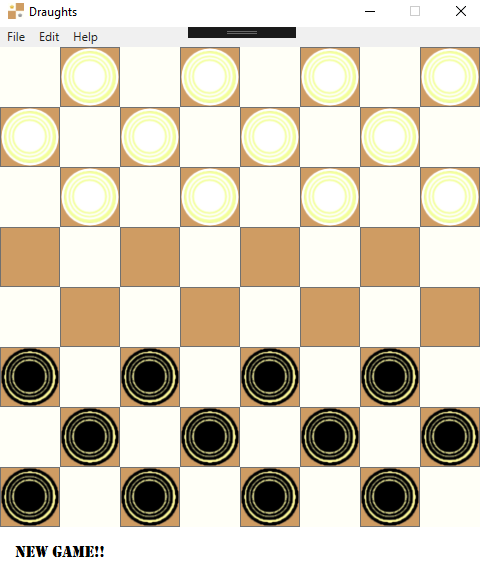
\includegraphics[scale = 0.4]{board}
  	\caption{Board and Markers - GUI of game board with markers ready to play}
  	\label{fig:nonfloat}
	\end{figure}

	I started with board which I made using a 2d array 8,8 so each square could be assigned to a number(-1 for invalid squares, 0 for empty squares, 1 White markers, 2 Black markers, 3 White kings, 4 Black kings) after the board was created I moved on to placing the markers, at this point I found a GUI was a better representation. I recreated the board using stack-panels still with the same numbering system.
	\subsection{Markers}
	I moved on placing markers on the board I used a case a statement to place them i felt this was a more effective than a series of if statements, The marker class contains 3 values the markers row and column and wither or not it has been promoted to a king. Then they get added to a stack panel.
	\subsection{Player vs Player}
I decided the best approach was to build working game first for player vs player, then sort out an AI player.  
	\subsection{Undo/Redo}
	To make my Undo/Redo Feature work I implemented four stacks. The undo feature uses Stacks after a player has preformed a move the move markers before and after position is added the a stack. if a marker was taken that markers co-ordinates re added to a taken marker stack so they can be replaced when a move is redone. The redo stack is added to after a move is undone and the retaken stack. After 
	\subsection{AI}
	\subsection{Game Replay}
	uses 1 queue and 2 stacks 

	\section{Enhancements}
	Some common formatting you may need uses these commands for \textbf{Bold Text}, \textit{Italics}, and \underline{underlined}.

	\section{Critical Evaluation}
	Some common formatting you may need uses these commands for \textbf{Bold Text}, \textit{Italics}, and \underline{underlined}.

	\section{Persona Evaluation}
	Some common formatting you may need uses these commands for \textbf{Bold Text}, \textit{Italics}, and \underline{underlined}.
	
    
    Here is a line followed by a double line break.
	This line is only one line break down from the above, Notice that latex can ignore this
    
    We can force a break \\ with the break operator.
   


		
\end{document}